\documentclass{beamer}

\usepackage{beamerthemesplit}
\usetheme{Singapore} %Copenhagen}
%\usecolortheme{whale}

%\usepackage[T2A]{fontenc}
%\usepackage[utf8]{inputenc}
%\usepackage[russian]{babel}

\usepackage[main=russian,english]{babel}   %% загружает пакет многоязыковой вёрстки
\usepackage{fontspec}      %% подготавливает загрузку шрифтов Open Type, True Type и др.
\defaultfontfeatures{Ligatures={TeX},Renderer=Basic}  %% свойства шрифтов по умолчанию
\setmainfont{Times New Roman} %% задаёт основной шрифт документа
%\usefonttheme{professionalfonts}% SOLUTION
\usefonttheme{serif}

\usepackage{hyperref}
\usepackage{textcomp}
\usepackage{amssymb,amsmath}
%\usepackage{animate}
%\usepackage{longtable}
\usepackage{xcolor}

%\usepackage{pgffor}
\usepackage{enumitem}
\usepackage[export]{adjustbox}

\newcounter{N}

%% Форматирование окружения itemize
%\usepackage{ragged2e}
%\let\olditem\item
%\renewcommand\item{\olditem\justifying}

\usepackage{ mathrsfs }
\newcommand{\Rho}{\mathscr{P}}

\newcommand{\argxi}{(\xi^1,\xi^2,\xi^3)}
\newcommand{\argx}{(x^1,x^2,x^3)}

\newcommand{\argxiv}{(\vec{\xi})}
\newcommand{\argxv}{(\vec{x})}


\newcommand{\argxbarn}{(\bar{x}^1,\bar{x}^2,\ldots, \bar{x}^n)}
\newcommand{\argxn}{(x^1, x^2,\ldots, x^n)}

\newcommand{\argtxi}{(t, \xi^1,\xi^2,\xi^3)}
\newcommand{\argtoxi}{(t_0, \xi^1,\xi^2,\xi^3)}

\newcommand{\argtxiv}{(t, \vec{\xi})}
\newcommand{\argtoxiv}{(t_0, \vec{\xi})}


\newcommand{\argtx}{(t, x^1,x^2,x^3)}
\newcommand{\argtox}{(t_0, x^1,x^2,x^3)}

\newcommand{\argtxv}{(t, \vec{x})}
\newcommand{\argtoxv}{(t_0, \vec{x})}


\newcommand{\pd}[2]{\frac{\partial #1}{\partial #2}}
\newcommand{\pdk}[2]{\frac{\partial^2 #1}{\partial #2^2}}

\newcommand{\od}[2]{\frac{d #1}{d #2}}

\newcommand{\grad}{\operatorname{grad}}
\newcommand{\rot}{\operatorname{rot}}
\newcommand{\divo}{\operatorname{div}}

\title[]{Плоские потенциальные течения идеальной жидкости}

\author[]{ {\em Верещагин Антон Сергеевич}
\\
канд. физ.-мат. наук, старший преподаватель\\
\bigskip
Кафедра аэрофизики и газовой динамики ФФ НГУ}

\usebackgroundtemplate{
\includegraphics[width=\paperwidth]{../img/background.png}}

\begin{document}
	
\frame{\titlepage}


\frame{
	\frametitle{Аннотация}
	\parbox{\textwidth}{
	 Определение плоского течения. Функция тока и её свойства. Связь потенциала и функции тока. Комплексный потенциал и его свойства. Простейшие течения.
	}
}

\frame{
	\frametitle{ Уравнения плоского течения идеальной жидкости }
	
	
	\parbox{\textwidth}{
		
	
	Если можно ввести систему координат так, что течение идеальной жидкости ($\rho=const$) будет описываться уравнениями	
	\[
		\pd{v_x}{x}+\pd{v_y}{y} = 0,	
	\]
	\[
		\pd{v_x}{t}+v_x \pd{v_x}{x} + v_y \pd{v_x}{y} = -\frac{1}{\rho} \pd{p}{x},
	\]
	\[
		\pd{v_y}{t}+v_x \pd{v_y}{x} + v_y \pd{v_y}{y} = -\frac{1}{\rho} \pd{p}{y},	
	\]
	где $v_x = v_x(t,x,y)$, $v_y = v_y(t,x,y)$, $p=p(t,x,y)$, то говорят, что движение идеальной жидкости \alert{плоскопараллельное}.
	
	}

}

\frame{
	\frametitle{ Функция тока }
	
	\begin{exampleblock}{Определение}
		\parbox{\textwidth}{
			Функция $\psi=\psi(x,y)$ такая, что 
			\[
			v_x = \pd{\psi}{y},\quad
			-v_y = \pd{\psi}{x},
			\]
			называется \alert{функцией тока}. Если течение нестационарное, то $t$ -- дополнительный параметр.
			
		}
	\end{exampleblock}
}

\frame{
	\frametitle{  Функция тока: уравнение неразрывности}
	
	\begin{exampleblock}{Уравнение неразрывности}
		\parbox{\textwidth}{
			
			Уравнение 
			\[
				\pd{v_x}{x} + \pd{v_y}{y} = 
				\pd{}{x} \left( \pd{\psi}{y} \right) + \pd{}{y} \left( -\pd{\psi}{x} \right) = 0
			\]
			выполняется тождественно.
			
			
		}
	\end{exampleblock}
}

\frame{
	\frametitle{  Функция тока:  линии тока }
	\parbox{\textwidth}{
	Рассмотрим уравнения линий тока
	\[
	\frac{dx}{v_x} = \frac{dy}{v_y},
	\]
	тогда
	\[
		0 = -v_y dx + v_x dy = \pd{\psi}{x} dx + \pd{\psi}{y} dy =  d\psi.
	\]
	Таким образом, $\psi=\psi(x,y)$ \alert{сохраняет} одно и тоже значение \alert{на линиях тока}.
		
	}
	
}

\frame{
	\frametitle{ Функция тока: поток жидкости  }
	

	\begin{columns}
		\begin{column}{0.45\textwidth}
			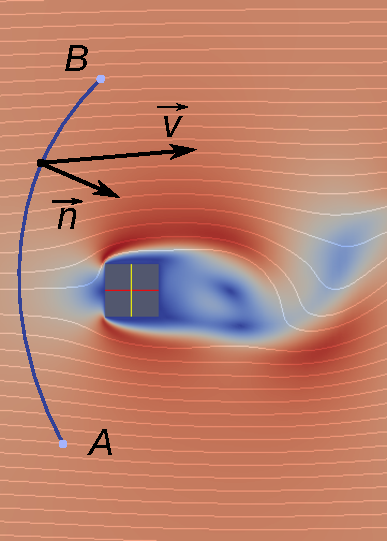
\includegraphics[width=\textwidth,frame]{../img/square_streamlines.pdf}					
		\end{column}
		\begin{column}{0.55\textwidth}
			\[
			\int\limits_B^A \vec{v}\cdot\vec{n} ds = 
			\int\limits_B^A \left( v_x n_1 + v_y n_2 \right) ds = 
			\]
			\[
			=
			\int\limits_0^{s_0} \left( \pd{\psi}{y} \pd{y}{s} + \pd{\psi}{x} \pd{x}{s} \right) ds=
			\]
			\[
			=
			\int\limits_0^{s_0} \frac{d}{ds} \psi(x(s),y(s)) ds = \psi(A) - \psi(B),
			\]
			\[
				x=x(s),\quad y=y(s),
			\]
			\[
				(x,y)|_{s=0} = B,\quad
				(x,y)|_{s=s_0} = A.
			\]
		\end{column}
	\end{columns}

}


\frame{
	\frametitle{ Функция тока: вектор вихря }
	
	\parbox{\textwidth}{
	Вектор вихря $\vec{\Omega}= \rot \vec{v}$ задаётся формулами
	\[
	\Omega_x = \pd{v_z}{y}-\pd{v_y}{z} = 0,\quad
	\Omega_y = \pd{v_x}{z}-\pd{v_z}{x} = 0,
	\]
	\[
	\Omega_z = \pd{v_y}{x}-\pd{v_x}{y} = -\pdk{\psi}{x} - \pdk{\psi}{y}.
	\]
	
	\pause\bigskip
	В случае безвихревого течения
	\[
	\Delta \psi = \pdk{\psi}{x} + \pdk{\psi}{y} = 0.
	\]
	}
	
	
}

\frame{
	\frametitle{ Связь потенциала и функции тока }
	
	\parbox{\textwidth}{
	Если плоское течение идеальной жидкости потенциально, тогда существует функция $\varphi(x,y)$, такая что
	\[
	v_x = \pd{\varphi}{x},\quad
	v_y = \pd{\varphi}{y}, 
	\]
	при этом
	\[
		\pd{\psi}{y} = \pd{\varphi}{x},\quad
		-\pd{\psi}{x} = \pd{\varphi}{y}.
	\]
	
	\pause\medskip
	Иначе,
	\[
		\pd{\varphi}{x}\pd{\psi}{x} + \pd{\varphi}{y}\pd{\psi}{y} = 0.
	\]
	Отсюда следует, что линии $\varphi=const$ и $\psi=const$ \alert{ортогональны}. Такие $\varphi$ и $\psi$ называются \alert{сопряжёнными}.
	
	}
	
	
}

\frame{
	\frametitle{ Комплексная плоскость и комплексный потенциал }
	\begin{exampleblock}{Комплексный потенциал}
	\parbox{\textwidth}{
		Функции $\varphi$ и $\psi$ связаны между собой условием Коши-Римана, поэтому функция комплексного переменного $w = \varphi(x,y) + i \psi(x,y)$ является \alert{аналитической функцией} комплексного аргумента $z = x + i y$:
		\[
		w = f(x+iy) = \varphi(x,y) + i  \psi(x,y).
		\]
		
		Функция $w(z)$ -- называется \alert{комплексным потенциалом}.
		
	}
	\end{exampleblock}


	
}

\frame{
	\frametitle{ Комплексная скорость }
	
	\begin{exampleblock}{Свойство}
	\parbox{\textwidth}{
		Так как $w(z)$ -- аналитическая функция, то существует $dw/dz$:
		\[
			\od{w}{z} = \pd{\varphi}{x}+\pd{\psi}{x} i = 
			\pd{\varphi}{x}-\pd{\varphi}{y} i. 
		\]
		
		
		\pause
		\begin{columns}
			\begin{column}{0.7\textwidth}
				\parbox{\textwidth}{
				Следовательно,
				\[
				\od{w}{z}=v_x-i v_y.
				\]
				
				Если ввести \alert{комплексную скорость} как
				\[
					v(z) = v_x(x,y) + i v_y(x,y),
				\] 
				то
				\[
				\od{w}{z} = v^* = v_x - i v_y.
				\]
				}
			\end{column}
			\begin{column}{0.3\textwidth}
			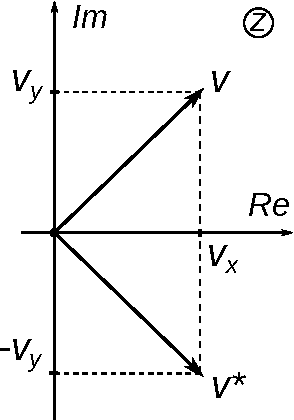
\includegraphics[width=\linewidth]{../img/v_star.pdf}
				
			\end{column}
		\end{columns}

		
		}
	\end{exampleblock}
}

\frame{
	\frametitle{ Связь плоской гидродинамической задачи с ТФКП  }
	
	\parbox{\textwidth}{
		Соотношение
		\[
		w = f(x+iy) = \varphi(x,y) + i  \psi(x,y).
		\]
		связывает аналитическую функцию $w(z)$ с определённой кинематической картиной течения, полем ($v_x$, $v_y$), с помощью аппарата теории функций комплексного переменного.
		
		\bigskip
		Рассмотрим простейшие примеры.
	}

}


\frame{
	\frametitle{ Однородное поступательное течение }
	\begin{exampleblock}{Комплексный потенциал}
		\parbox{\textwidth}{
			\[
			w(z) = a z,\quad
			a \in\mathbb{R}.
			\]

		}
	\end{exampleblock}
	\begin{exampleblock}{Комплексная скорость}
		\parbox{\textwidth}{
			\[
			\od{w}{z} = a = v_x - i v_y \Rightarrow
			v_x = a,\quad v_y = 0.
			\]
		}
	\end{exampleblock}


	
}

\frame{
	\frametitle{Однородное поступательное течение: картина течения }
			\centering
			\[
			a > 0
			\]
			
			\medskip
			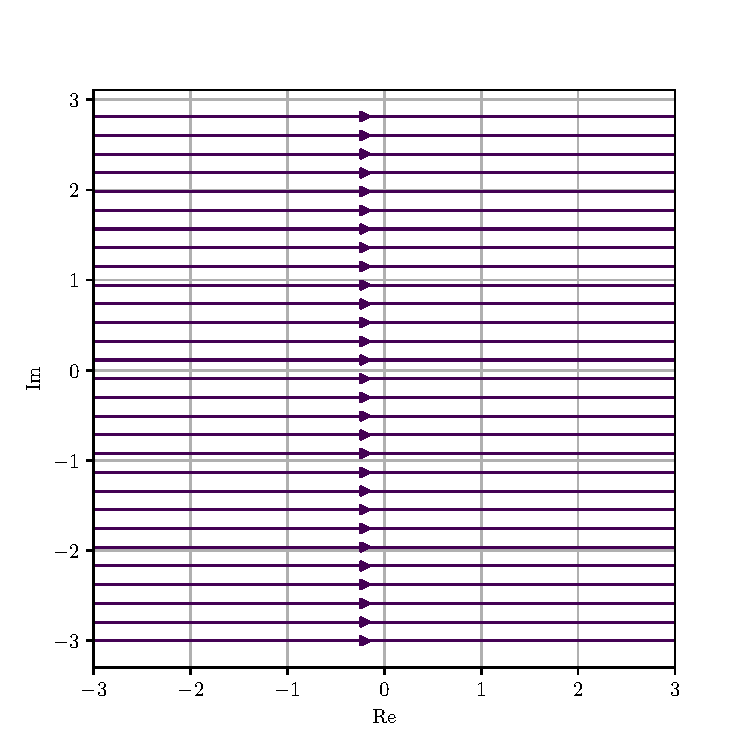
\includegraphics[width=0.55\textwidth]{../img/uniform_translation.pdf}
}


\frame{
	\frametitle{ Источник и сток }
	
	\begin{exampleblock}{Комплексный потенциал}
		\parbox{\textwidth}{
			\[
			w(z) = \frac{q}{2\pi}\ln(z-z_0),\quad
			q \in\mathbb{R}, z_0\in\mathbb{C}.
			\]
			
		}
	\end{exampleblock}
	\begin{exampleblock}{Комплексная скорость (при $z_0=0$)}
		\parbox{\textwidth}{
			Пусть $z=x+iy=re^{i\theta}$, тогда
			\[
			\od{w}{z} = \frac{q}{2\pi}\frac{1}{z} \Rightarrow
			\left\{
			\begin{array}{l}
			\displaystyle v_x = \frac{q}{2\pi}\frac{x}{x^2+y^2} = \frac{q}{2\pi}\cos\theta,\\
			\displaystyle v_y = \frac{q}{2\pi}\frac{y}{x^2+y^2} = \frac{q}{2\pi}\sin\theta.
			\end{array}
			\right.
			\]
		}
	\end{exampleblock}
	
	\begin{exampleblock}{Картина течения}
		\parbox{\textwidth}{
			Нарисовать картину течения при $q>0$ (источник) и $q<0$ (сток).
			
		}
	\end{exampleblock}
}

\frame{
	\frametitle{  Источник и сток: картина течения }
	
	\begin{columns}
	\begin{column}{0.5\textwidth}
			\centering
			Источник
			\[
			q > 0
			\]
			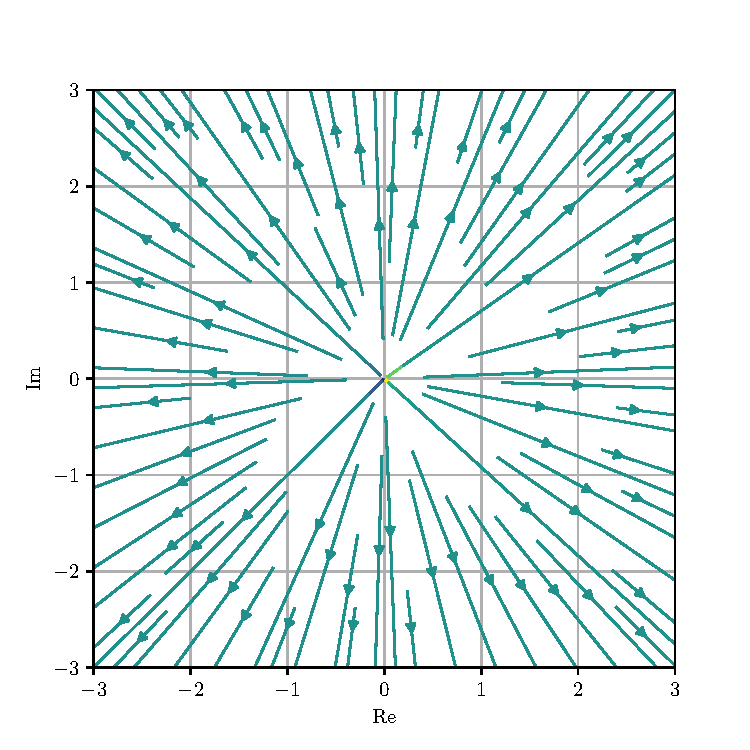
\includegraphics[width=\linewidth]{../img/source.pdf}
	\end{column}
	\begin{column}{0.5\textwidth}
			\centering
			Сток
			\[
			q < 0
			\]			
			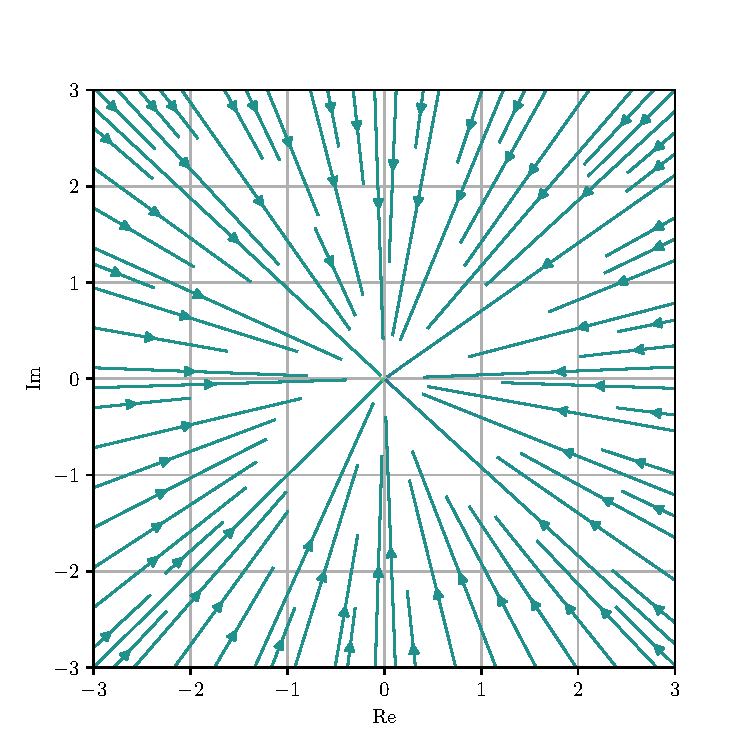
\includegraphics[width=\linewidth]{../img/sink.pdf}
			
		\end{column}
	\end{columns}
}


\frame{
	\frametitle{ Вихрь }
	
	\begin{exampleblock}{Комплексный потенциал}
		\parbox{\textwidth}{
			\[
			w(z) = \frac{\Gamma}{2\pi i}\ln(z-z_0),\quad
			q \in\mathbb{R}, z_0\in\mathbb{C}.
			\]
			
		}
	\end{exampleblock}
	\begin{exampleblock}{Комплексная скорость (при $z_0=0$)}
		\parbox{\textwidth}{
			Пусть $z=x+iy=re^{i\theta}$, тогда
			\[
			\od{w}{z} = \frac{\Gamma}{2\pi i}\frac{1}{z} \Rightarrow 
			\left\{
			\begin{array}{l}
		\displaystyle	v_x = -\frac{\Gamma}{2\pi i}\frac{y}{x^2+y^2} = -\frac{\Gamma}{2\pi i}\sin\theta,\\
		\displaystyle	v_y = \frac{\Gamma}{2\pi i}\frac{x}{x^2+y^2} = \frac{\Gamma}{2\pi i}\cos\theta.
			\end{array}
			\right.
			\]
		}
	\end{exampleblock}
	
	\begin{exampleblock}{Картина течения}
		\parbox{\textwidth}{
			Нарисовать картину течения при $\Gamma>0$ и $\Gamma<0$.
			
		}
	\end{exampleblock}
}

\frame{
	\frametitle{ Вихрь: картина течения}
	\begin{columns}
		\begin{column}{0.5\textwidth}
			\centering
			\[
			\Gamma > 0
			\]
			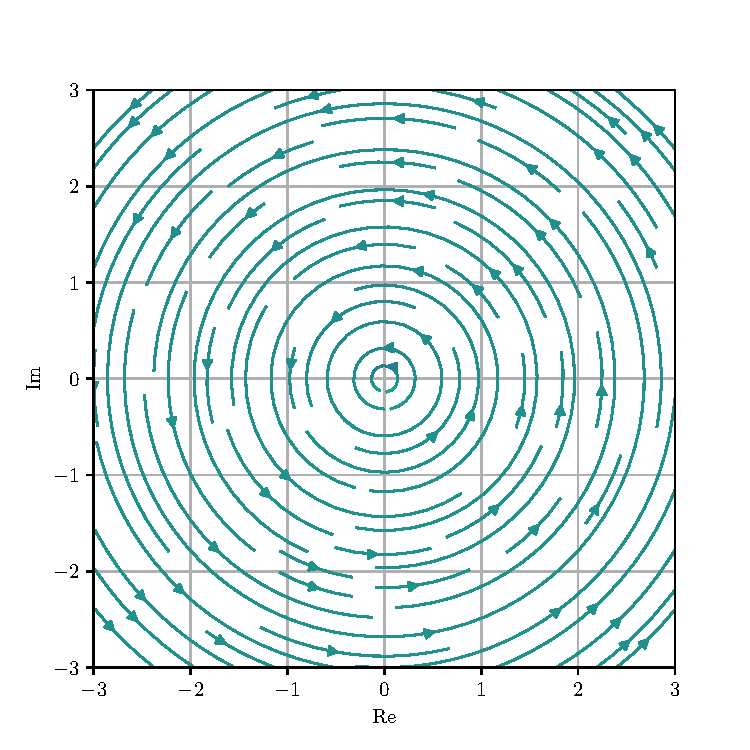
\includegraphics[width=\linewidth]{../img/rot_Gamma_g_0.pdf}
		\end{column}
		\begin{column}{0.5\textwidth}
			\centering
			\[
			\Gamma < 0
			\]			
			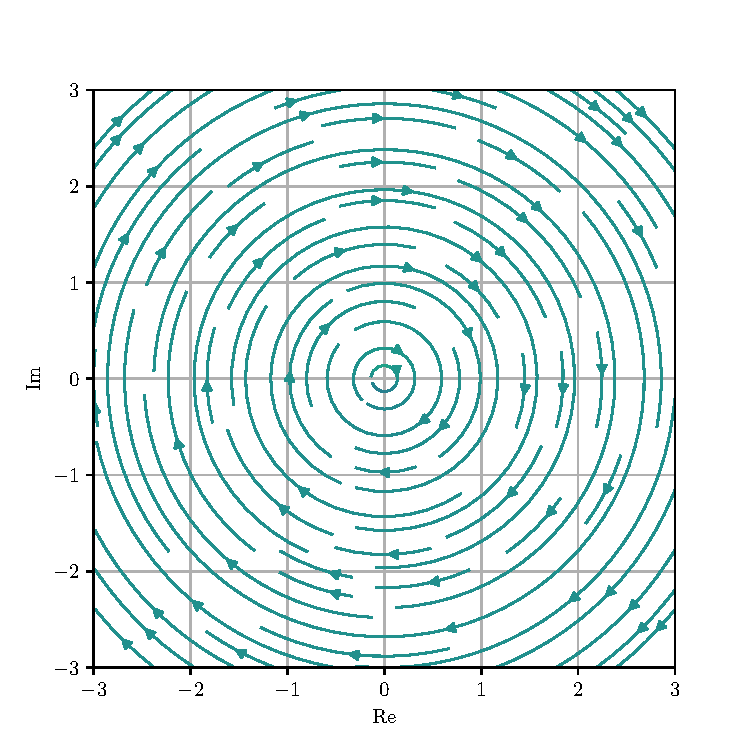
\includegraphics[width=\linewidth]{../img/rot_Gamma_l_0.pdf}
			
		\end{column}
	\end{columns}

}


\frame{
	\frametitle{ Диполь }
	
	\begin{exampleblock}{Комплексный потенциал}
		\parbox{\textwidth}{
			\[
			w(z) = \frac{D e^{i\alpha}}{2\pi z},\quad
			D,\alpha \in\mathbb{R}.
			\]
			
		}
	\end{exampleblock}
	\begin{exampleblock}{Комплексная скорость (при $\alpha=0$)}
		\parbox{\textwidth}{
			Пусть $z=x+iy=re^{i\theta}$, тогда
			\[
			\od{w}{z} = -\frac{D}{2\pi}\frac{1}{z^2} \Rightarrow\displaystyle
			\left\{
			\begin{array}{l}
			v_x = -\displaystyle\frac{D}{2\pi r^2} \cos 2\theta,\\
			v_y = -\displaystyle\frac{D}{2\pi r^2} \sin 2\theta.
			\end{array}
			\right.
			\]
		}
	\end{exampleblock}
	\begin{exampleblock}{Картина течения}
	\parbox{\textwidth}{
		Нарисовать картину течения.
		
	}
	\end{exampleblock}	
	
}

\frame{
	\frametitle{ Диполь: картина течения }

	\centering
	\[
	D > 0
	\]
	\medskip
	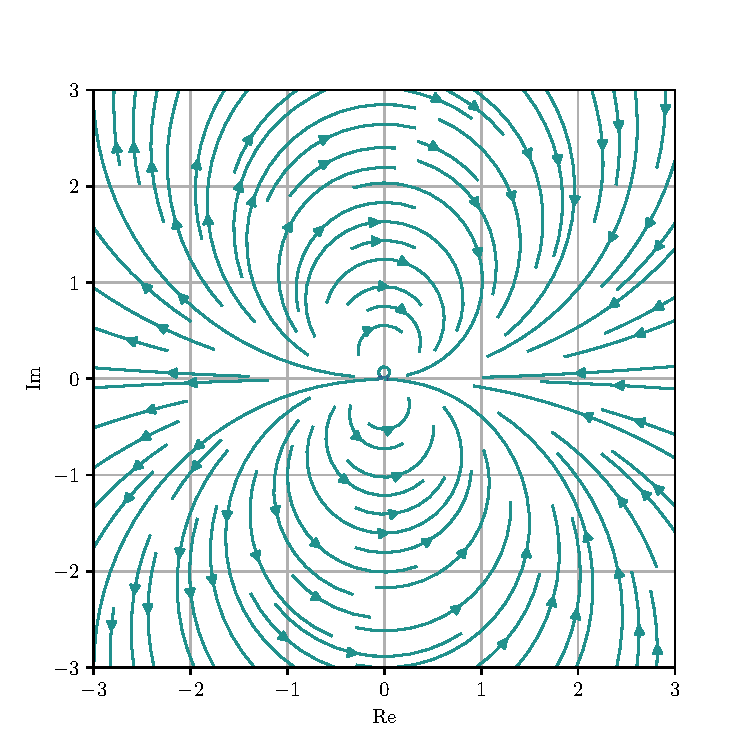
\includegraphics[width=0.6\linewidth]{../img/dipol.pdf}

}

\frame{
	\frametitle{ Принцип суперпозиций }
	
	\begin{exampleblock}{Утверждение}
		\parbox{\textwidth}{
			
			В следствие линейности уравнения неразрывности относительно потенциала, то если в области имеется несколько течений с потенциалами $w_1(z)$, $w_2(z)$, \ldots , $w_n(z)$, тогда общий потенциал всего течения в заданной точке равен сумме потенциалов всех течений, присутствующих в области
			\[
				w(z) = w_1(z) + w_2(z) + \ldots + w_n(z).
			\] 
			
		}
	\end{exampleblock}
	
}



\frame{
	\frametitle{ Литература }
	\begin{itemize}[partopsep=1pt,label=\textbullet]
		\item 
		{\em Кочин~Н.~Е., Кибель~И.~А., Розе~Н.~В.} Теоретическая гидромеханика. М.:Гос. издат. физ.-мат. лит., 1963.
	\end{itemize}
}

\end{document}